\chapter{Robust self-testing of two-qubit maximally entangled state}

In the previous chapter, we examined the self-test of a two-qubit maximally entangled state from correlations achieving a maximal violation of the CHSH inequality.
However, such correlations can hardly be observed experimentally. 
Indeed, imperfections such as noise and loss in creating, distributing and measuring the quantum state, will unavoidably lead to non-ideal correlations, i.e. not maximally violating the Bell inequality.
Furthermore, since any self-testing experiment can only collect a limited sample of Bell game rounds, the correlations are only estimated up to a certain confidence interval. %Yes we can remove but interval of confidence -> lower CHSH bound
Acknowledging such limitations, there is the need for self-testing protocols robust to the presence of imperfections in the correlations, also known as \textit{robust self-testing}.

There is multiple approaches to robust self-testing. 
Chronologically, the Mayers-Yao self-test was made robust in \cite{Magniez2006} while robust self-testing based on CHSH was introduced in \cite{Bardyn2009}.
A framework for the robust self-testing of the singlet was presented in \cite{McKague2012}.
Since then, numerous improvement were made to improve the robustness of self-testing, and to extended it to different scenario, e.g. Bell scenarios with more inputs or outputs.

Here we present a numerical method, using Jordan's lemma, relevant for the robust self-test of the singlet. 
Two notable methods than will not be discussed here are the analytical method based on operator inequalities presented in ~\cite{Kaniewski2016} and the numerical one SWAP method~\cite{Bancal2015}.
We then expose some fundamental limitations on robust self-testing based on the CHSH inequality.
Finally, we present a method that we developed, overcoming some of these limitations by extending robust self-testing of the singlet beyond the CHSH inequality.

\section{Extractability}

In robust self-testing, the goal is to use the correlations observed in a Bell game to bound the \textit{closeness} of the shared state, $\rho_{AB}$ to the target state $\ket{\psi_{AB}}$ that we here consider pure.
Similarly to ideal-case self-testing, Alice and Bob can craft local isometries, $f_A$ and $f_B$, to identify the relevant degree of freedom from the shared state encoding the target state.
Taking into account local isometries, a possible notion of \textit{closeness} is the so-called \textit{extractability} expressed as
\begin{equation}
	\Xi [\rho_{AB} \rightarrow \psi_{AB}] = \sup_{\{f_A,f_B\}} F((f_A \otimes f_B)[\rho_{AB}],\psi_{AB} \otimes \varrho_\text{junk})
	\label{eq:extractability_junk}
\end{equation}
where $F(\rho_0,\rho_1) = \left(\trr{\sqrt{\rho_0^{1/2}\rho_1\rho_0^{1/2}}}\right)^2$ is the square of the Uhlmann fidelity, which reduces to the overlap $F(\rho_0,\rho_1)=\trr{\rho_0\,\rho_1}$ if any of the two states is pure.
The separable state $\psi_{AB} \otimes \varrho_\text{junk}$ consists of $\psi_{AB} = \ketbra{\psi_{AB}}$, the target state, and $\varrho_\text{junk}$ containing all remaining degrees of freedom which can be traced out.
As an isometry mapping a state from one hilbert space $\Hil_1$ to another $\Hil_2$ can be thought of as a unitary operation on $\Hil_1 \otimes \Hil_2$ before discarding the susbytem laying on $\Hil_1$, we can rewrite the extractability as
 
\begin{equation}
	\Xi [\rho_{AB} \rightarrow \psi_{AB}] = \sup_{\{\Lambda_A,\Lambda_B\}} F((\Lambda_A \otimes \Lambda_B)[\rho_{AB}],\psi_{AB}).
	\label{eq:extractability}
\end{equation}
where $\Lambda_A,\Lambda_B$ are \acrfull{CPTP} maps. 
A detailed proof of the equivalence of these two extractability definitions in case the target state is pure can be found in \cite{Sekatski2018}.


Note that the extractability is lower bounded by $1/2$ as it is always possible for Alice and Bob to construct maps discarding the received state and preparing a new one with a fidelity of $1/2$ with respect to the target one. 
For example, if the target state is the singlet $\psi^{-}$, we can build maps acting as
\begin{equation}	
	\left(\Lambda_A \otimes \Lambda_B\right)[\rho_{AB}] = \ket{1}\bra{1} \otimes \ket{0}\bra{0}.
\end{equation}
Therefore, a non-trivial self-testing statement can be made if and only if $\Xi[\rho_{AB}]>1/2$.


\section{Robustness of CHSH-based singlet self-tests}

\subsection{Robust self-testing with two binary measurements}

As a device-independent protocol, no assumption is made on the dimension of the shared quantum state and the measurements.
However, in the particular case of a Bell game where Alice and Bob own two dichotomic measurements, i.e. with two outcomes, we can use Jordan's lemma to define a basis where local observables are block diagonal.
Indeed, Jordan's lemma states that for two Hermitian operators with eigenvalues $\pm1$ there exists a basis in which both operators are block-diagonal, with blocks of dimension $2 \times 2$.
To simplify further calculations, we consider these blocks to be in the $(\sigma_x,\sigma_z)$-plane.
This is done without loss of generality as Alice and Bob can always perform local rotations of their basis to recover that plane.
Alice and Bob observables can thus be written as a direct sum over these blocks 
\begin{equation}
	\begin{split}
	A_x = \bigoplus_i A_x^i &= \bigoplus_i \cos(\alpha_i)\sigma_h + (-1)^x \sin(\alpha_i)\sigma_m, \\
	B_y = \bigoplus_j B_y^j &= \bigoplus_j \cos(\beta_j)\sigma_z + (-1)^y \sin(\beta_j)\sigma_x,
	\end{split}
	\label{eq:block_observables}
\end{equation}
with $\sigma_{m,h} = (\sigma_z \pm \sigma_x)/\sqrt{2}$ and for some measurement angles $\alpha_i,\beta_j\in[0,\pi/2]$ for each block, indexed by $i$ and $j$.
Trivially, the CHSH operator defined in \refeq{CHSH_operator} inherits the same block structure and can be express following
\begin{equation}
	\mathcal{B}_\text{CHSH} = \bigoplus_{i,j} \mathcal{B}_\text{CHSH}^{i,j} = \bigoplus_{i,j} A_0^i \otimes (B_0^j + B_1^j) + A_1^i (B_0^j - B_1^j).
	\label{eq:block_operator}
\end{equation}

The shared quantum state $\rho_{AB}$ does not necessarily have a block diagonal structure. 
However, before measuring this state, Alice and Bob can always project it in their respective local basis to obtain the state
\begin{equation}
	\tilde{\rho}_{AB} = \bigoplus_{i,j} p_{i,j}\rho_{AB}^{i,j}
\end{equation}
where $p_{i,j}$ is the success probability to project $\rho_{AB}$ in the $(i,j)$-block.
Note that the state $\tilde{\rho}_{AB}$ achieve the same CHSH violation as $\rho_{AB}$ thanks to the block structure of the CHSH operator
\begin{equation}
	S = \trr{\mathcal{B}_\text{CHSH}\rho_{AB}} = \sum_{i,j} p_{i,j} \trr{\mathcal{B}_\text{CHSH}^{i,j}\rho_{AB}^{i,j}}.
\end{equation}

In the previous chapter, we have seen that in order to complete a self-testing statement we need to construct local maps $\Lambda = \Lambda_A \otimes \Lambda_B$.
These local isometries can be constructed using the same block diagonal recipe 
\begin{equation}
		\Lambda = \bigoplus_{i,j} \Lambda_A^i \otimes \Lambda_B^j
\end{equation}
with the isometry in each block acting as
\begin{equation}
	\Lambda_A^i: \mathcal{L}(\mathds{C}^2) \rightarrow \mathcal{L}(\mathds{C}^2), \qquad \Lambda_B^j: \mathcal{L}(\mathds{C}^2) \rightarrow \mathcal{L}(\mathds{C}^2).
\end{equation}

From this block structure, the singlet extractability defined in \eqref{eq:extractability} reads
\begin{equation}
	\Xi [\rho_{AB} \rightarrow \psi^{-}] = \sup_{\{\Lambda_A^i,\Lambda_B^j\}} \sum_{i,j} p_{i,j} F((\Lambda_A^i \otimes \Lambda_B^j)[\rho_{AB}^{ij}],\psi^{-}).
	\label{eq:block_extractability}
\end{equation}
Given that the probabilities $p_{i,j}$ are non-negative real numbers that sum up to $1$, by definition, the singlet extractability is given by a convex sum of the singlet extractability on two-qubit blocks.

\medbreak

To obtain a CHSH-based robust self-test of the singlet, we need to lower bound the singlet extractability with respect to all quantum realization achieving a given CHSH score $S$.
In order to do so, we can first obtain a lower bound on this extractability over all two-qubit blocks.
This can be done by first fixing the dependence of the maps on the block indexes $(i,j)$.
Note that the resulting isomteries might not maximizes the singlet extractability.
Therefore, we will obtain a lower bound on \refeq{block_extractability} in this way.
The minimum singlet fidelity over all two-qubit states and measurement choices compatible with a score $S$ is obtained by solving the optimisation
\begin{equation}
	\begin{split}
		O_{\min}(S)=\min_{i, j, \tau} \-\ & F(\Lambda_A^i \otimes\Lambda_B^j [\tau] ,\psi^-)\\
		\text{s.t.} \-\ &\trr{\mathcal{B}_{CHSH}^{i,j}\, \tau} \geq S,\\
		& \tau \geq 0,\\
		& \tr{(\tau)} =1,\\
		& \tau^\dag = \tau.
	\end{split}
	\label{eq:sdp_extractability}
\end{equation}
The optimisation over all two-qubit states $\tau$ can be solved to arbitrary precision using semi-definite programming (see Appendix), while the optimisation over the blocks indexes is a non-linear optimisation over measurement angles.

Using the convex structure of \refeq{block_extractability}, the convex roof of $O_{\min}(S)$ over all CHSH scores, $f(S)$, gives a lower bound on the singlet-extractability with respect to the CHSH score~\cite{Sekatski2018}.
Therefore, from a CHSH score $S$, one can hope to extract a singlet fidelity of at most 
\begin{equation}
	\Xi [\rho_{AB} \rightarrow \psi^{-}] \geq \mathcal{F}(S)=\max\left(1/2, f(S)\right).
\end{equation}

\subsection{Robustness bounds}

% Should I really get rid of this?
To asses the performance of robust self-testing, we are interested in the evolution of the extractability with respect to the Bell violation.
In particular, the minimum violation for which a non-trivial fidelity to the target state can be extracted is called the \textit{robustness bound}.
This bound is crucial as any implementation of a self-testing protocol is required to have the capabilities to achieve a Bell violation at least as high as the robustness bound.

To glean the robustness bound with the method presented in the previous section, we first need to choose the local isometries $\Lambda_A^i$ and $\Lambda_B^i$ appearing in \refeq{sdp_extractability}.
These isometries are completely-positive trace preserving maps acting on qubit space and parametrised by Alice and Bob measurement choice, respectively.
A relevant pick for such maps has been reported in \cite{Kaniewski2016}.
For the block $i$, let Alice's map be a dephasing map of the form
\begin{equation}
	\Lambda_A^i(\alpha_i)[\rho_{AB}] = \left( \frac{1+g(\alpha_i)}{2}\id\rho_{AB}\id+\frac{1-g(\alpha_i)}{2}\Gamma(\alpha_i)\rho_{AB}\,\Gamma(\alpha_i)\right),
	\label{eq:dephasing_maps}
\end{equation}
with a dephasing strength
\begin{equation}
	g(\alpha_i)=(1+\sqrt{2})(\cos{\alpha_i}+\sin{\alpha_i}-1)
	\label{eq:dephasing_strength}
\end{equation}
and a dephasing direction
\begin{equation}
	\Gamma(\alpha_i) = \begin{cases}
      \sigma_h, & \text{if}\ \alpha_i\leq\frac{\pi}{4} \\
      \sigma_m, & \text{otherwise}.
    \end{cases}
	\label{eq:dephasing_direction_alice}
\end{equation}
For the block $j$ and the corresponding measurement angle $\beta_j$, Bob's map is of the same form, but with a dephasing direction given by
\begin{equation}
	\Gamma(\beta_j) = \begin{cases}
      \sigma_h, & \text{if}\ \beta_j\leq\frac{\pi}{4} \\
      \sigma_m, & \text{otherwise}.
    \end{cases}
	\label{eq:dephasing_direction_bob}
\end{equation}

We can now solve the optimisation \refeq{sdp_extractability} to get $O_{\min}(S)$ and, from the convex roof, obtain $\mathcal{F}(S)$, the lower bound on the singlet extractability as a function of the CHSH score.
These functions are depicted in \reffig{fidCHSH}.
A non-trivial fidelity is achieved for any CHSH violation greater than $S \approx 2.11$, the robustness bound. 

It is worth noting that, using an analytical approach~\cite{Kaniewski2016}, this bound has been found at $S=(16+14\sqrt{2})/17\approx2.11$, compatible with the numerical result we present here.

\begin{figure}
	\begin{center}
		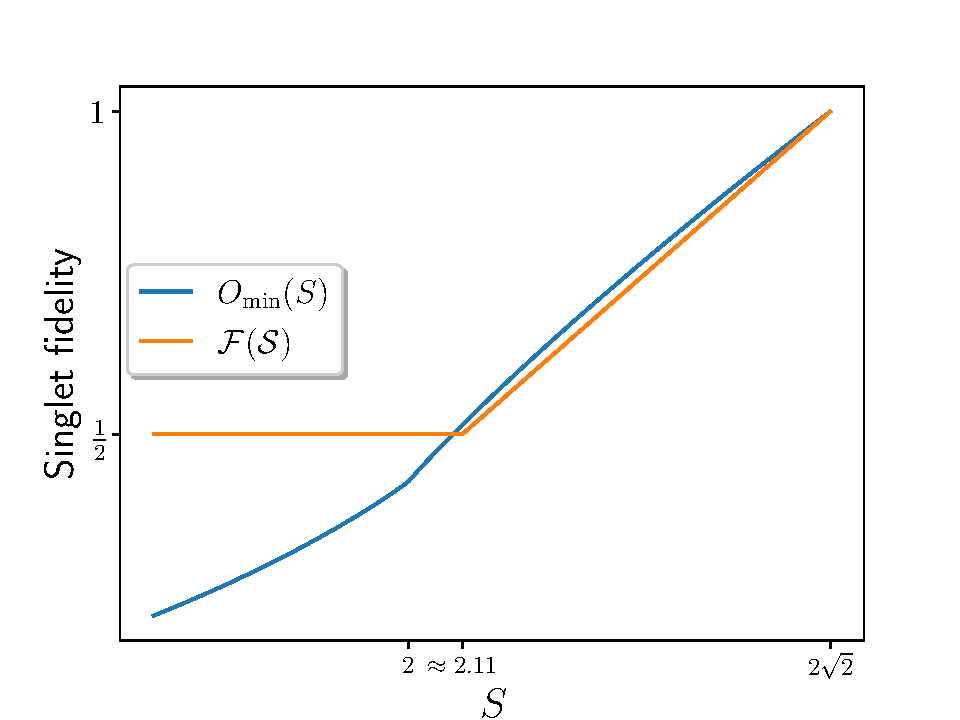
\includegraphics[width=0.95\textwidth]{chapters/selftesting/img/fidCHSH.pdf}
	\end{center}
	\caption{Lower bound on the singlet extractability with respect to the CHSH score $S$.}
	\label{fig:fidCHSH}
\end{figure}

\subsection{Limits of CHSH-based singlet self-testing}

While continuous efforts are made to improve the robustness bound of CHSH-based self-testing, another approach focuses on finding the \textit{threshold CHSH score} below which no self-testing statement can be made.
Surprisingly, it has been demonstrated~\cite{Coopmans19} that this threshold does not coincide with the local bound $S=2$.
The demonstration is based on an example of a state achieving a CHSH score of $S=2.0014$ while having a singlet extractability of $1/2$.

\medbreak

There is thus a threshold CHSH score higher than the local bound $2$ and lower than $2.11$, below which it is not possible to get a non-trivial self-testing statement.
This raises numerous questions. 
First, as photonic implementations seems more desirable for technological applications of self-testing, most photonic loop-hole free Bell test realisation are based on polarization entangled photons for which detection efficiencies of $\approx 90\%$ are required to achieve a score higher that $2.11$~\cite{Vivoli2015b}. 
Such detection efficiencies are beyond the realm of current possibilities. 
Therefore, if the threshold CHSH score is close to $2.11$, self-testing the singlet will be hard to perform experimentally with photonic realization.
In the opposite, if that threshold is close to the local bound, efforts are needed to craft better local maps than the ones proposed in Ref.~\cite{Kaniewski2016}.
Thirdly, and more fundamentally, it raises the question of the type of resources needed for self-testing.

The CHSH threshold prove that under local operation (LO) only, singlet-extraction is not possible from any CHSH violation.
However, if Alice and Bob can share classical information (LOCC), a singlet state can always be extracted from the slightest CHSH violation~\cite{Bardyn2009}. 
Therefore, it would be interesting to explore if this threshold still occurs under other regimes such as local operations and shared randomness (LOSR).
%Finally, it is worth exploring whether this threshold appears when the singlet-fidelity in the extractability is replaced by another quantity such as the trace distance. 

\medbreak

In an attempt to answer some of these question, in Article 1~\cite{Valcarce2020} we search for the quantum realization achieving a maximum CHSH score while resulting in a trivial singlet extractability.
Using Jordan's lemma, this problem correspond to the optimization
\begin{equation}
	\begin{split}
		\sup_{\{\rho_{AB},A_x,B_y\}}\ &S=\sum_{i,j} p_{i,j} \tr (\mathcal{B}_\text{CHSH}^{i,j} \rho_{AB}^{i,j})\\
\textnormal{s.t.}\ &\,\Xi[\rho_{AB}\rightarrow \psi^-] \leq \frac{1}{2} \\
				   &\, \rho_{AB} = \bigoplus_{i,j} \rho_{AB}^{i,j} = \sum_{ij} \ketbra{i} \otimes \ketbra{j} \otimes \rho_{AB}^{i,j} \\
				   &\, A_x = \bigoplus_{i} A_x^i = \sum_{i} \ketbra{i} \otimes A_x^{i} \\
				   &\, B_y = \bigoplus_{j} B_y^j = \sum_{j} \ketbra{j} \otimes B_y^{j}
	\end{split}
	\label{eq:CHSH_threshold}
\end{equation}
This problem is hard to tackle as for every quantum realization we need to obtain a certified upper-bound on the singlet extractability.
Since the extractability consists of a non-linear optimisation over CPTP maps, the certification of a tight upper-bound can not be guaranteed.

Therefore, as the proof can be constructive, we choose to limit ourselves to a subset of this problem.
First, following the intuition behind \cite{Coopmans19}, we limit ourselves to the case of three two-qubit blocks per party, i.e. $i,j=\{1,2,3\}$.
We consider observables with $2 \times 2$ blocks defined as 
\begin{equation}
	\begin{split}
		A_0^i = \sigma_z, &\quad A_1^i \in \{\sigma_z,\sigma_x,-\sigma_z\}_{i=1}^3  \\
		B_0^j = \sigma_h, &\quad B_1^j \in \{\sigma_h,\sigma_m,-\sigma_h\}_{j=1}^3 
	\end{split}
\end{equation}
where $\sigma_{h,m} = (\sigma_z\pm\sigma_x)/\sqrt{2}$.
We focus on a family of state that are a mixture between the singlet state and separable states build from the structure of the Bell operator
\begin{equation}
	\rho_{AB} = \nu \left(\ketbra{2} \otimes \ketbra{2} \otimes \rho_{AB}^{2,2}\right) 
	+ (1-\nu) \sum_{i,j \neq \{2,2\}} p_{i,j} \ketbra{i} \otimes \ketbra{j} \otimes \rho_{AB}^{i,j}
\end{equation}
with 
\begin{equation}
	\begin{split}
    \rho_{AB}^{2,2}&=\ketbra{\psi^-} \\
    \rho_{AB}^{3,2}&= \frac{1}{4}(\id\otimes \id +\sigma_z\otimes \sigma_m)\\
    \rho_{AB}^{3,3}&= \frac{1}{4}(\id-\sigma_z)\otimes(\id+\sigma_h)\\
    \rho_{AB}^{1,1}=\rho_{AB}^{1,3}=\rho_{AB}^{3,1} &= \frac{1}{4}(\id+\sigma_z)\otimes(\id+\sigma_h),
	\end{split}	
\end{equation}
and with $p_{i,j} =0$ for all other values of $i,j$.
Conveniently, this family of states yield a CHSH score of $S=2+(2\sqrt{2}-2)\nu$.

A relaxation of all separable two-qubit maps on these specific states, which we detailed in our article, allow us to obtain an upper bound on the singlet extractability given as a non-linear maximisation of only five real parameters.
To obtain a CHSH threshold, we minimized this upper-bound over the weights of the states of the family we consider, for a gradually increasing CHSH score, i.e. for a higher $\nu$.
This approach gave us a state with a parameter $\nu=0.061$, hence achieving a CHSH violation of $\approx 2.05$, from which non singlet can be extracted.
Our result pushed the CHSH threshold by an order of magnitude.
Importantly, this show the limitation of CHSH-based self-testing as the \textit{CHSH threshold} lays in the $[2.05,2.11]$ range.


\section{Robust singlet self-testing beyond CHSH}

In an attempt to make robust self-testing more accessible to experimental implementations, there is the need for protocols more resistant to noises and losses.
In the previous section, we saw that robust CHSH-based self-testing has been only proven for a CHSH score higher than $S\approx 2.11$ and can not be made for score below $2.05$.
These relatively high CHSH score are hardly in reach experimentally, and, as such, a very few self-testing experiments have been reported so far~\cite{Tan2017,Bancal2021}.

It is in this scope that in Article 2 we proposed a new protocol for robust self-testing.
Our approach is based on a more refined analysis of the correlations which are needed to compute the CHSH score, i.e. our protocol does not require any additional data.
Instead of using a single Bell inequality, our protocol relies on a family of \textit{generalized CHSH inequalities}
\begin{equation}
S_\theta = \sqrt{2}(\cos(\theta) \underbrace{\mean{A_0(B_0+B_1)}}_{X} + \sin(\theta)\underbrace{\mean{A_1(B_0-B_1)}}_{Y})
\end{equation}
parametrized by an angle $\theta \in [0,\pi/2]$, for which we derived robust self-testing statements.

As our approach applies to a Bell game with two dichotomic measurements, we proved self-testing statements from Jordan's lemma, following the steps explained in the previous section. 
Analogously to the CHSH-case, we obtained the robustness bound by minimizing the singlet fidelity over all state and measurement choices, for fixed maps.
We crafted maps with a dependency in both the local measurement choice and $\theta$.
More specifically, these maps are inspired by the one presented in \refeq{dephasing_maps}, with a couple of tweaks, notably a dephasing strength depending on $\theta$, and for one party, an additional rotation along $\sigma_y$ as well as a dephasing direction depending on the angle of measurement and $\theta$.

We then provide a robust self-testing statement recipe for any given correlator pair $(X,Y)$.
From a list of parameters $\theta$ and the corresponding robustness bound $S_\theta^\text{bound}$ that we provide, one can hope to obtain a singlet-extractability of 
\begin{equation}
	\max_\theta \mathcal{F}(S_\theta) = \max_\theta \left[ \begin{cases}
			\frac{1}{2},& \text{if} S_\theta \leq S_\theta^\text{bound}, \\
			\frac{1}{2}\left(1+\frac{S_\theta - S_\theta^\text{bound}}{2\sqrt{2}-S_\theta^\text{bound}}\right), & \text{otherwise}.
	\end{cases} \right]
	\label{eq:singlet-extractability-theta}
\end{equation}
The maximum singlet-extractability over all $\theta$, as a function of correlator pairs $(X,Y)$ is depicted in \reffig{generalizedCHSHfid}.

Comparing to CHSH-based self-testing, our protocol achieve higher singlet-extractability for any correlator $X\neq Y$.
Furthermore, our protocol can be used to perform self-tests for correlation leading to CHSH violation below the robustness bound of $S\approx 2.11$, below which no self-testing statement has been proven, and even below the currently known CHSH threshold of $2.05$, providing enough imbalance between the correlators, e.g. $X \gg Y$.
Therefore, this protocol makes self-testing implementations more accessible, especially in a case of imbalanced correlator.

\begin{figure}
	\begin{center}
		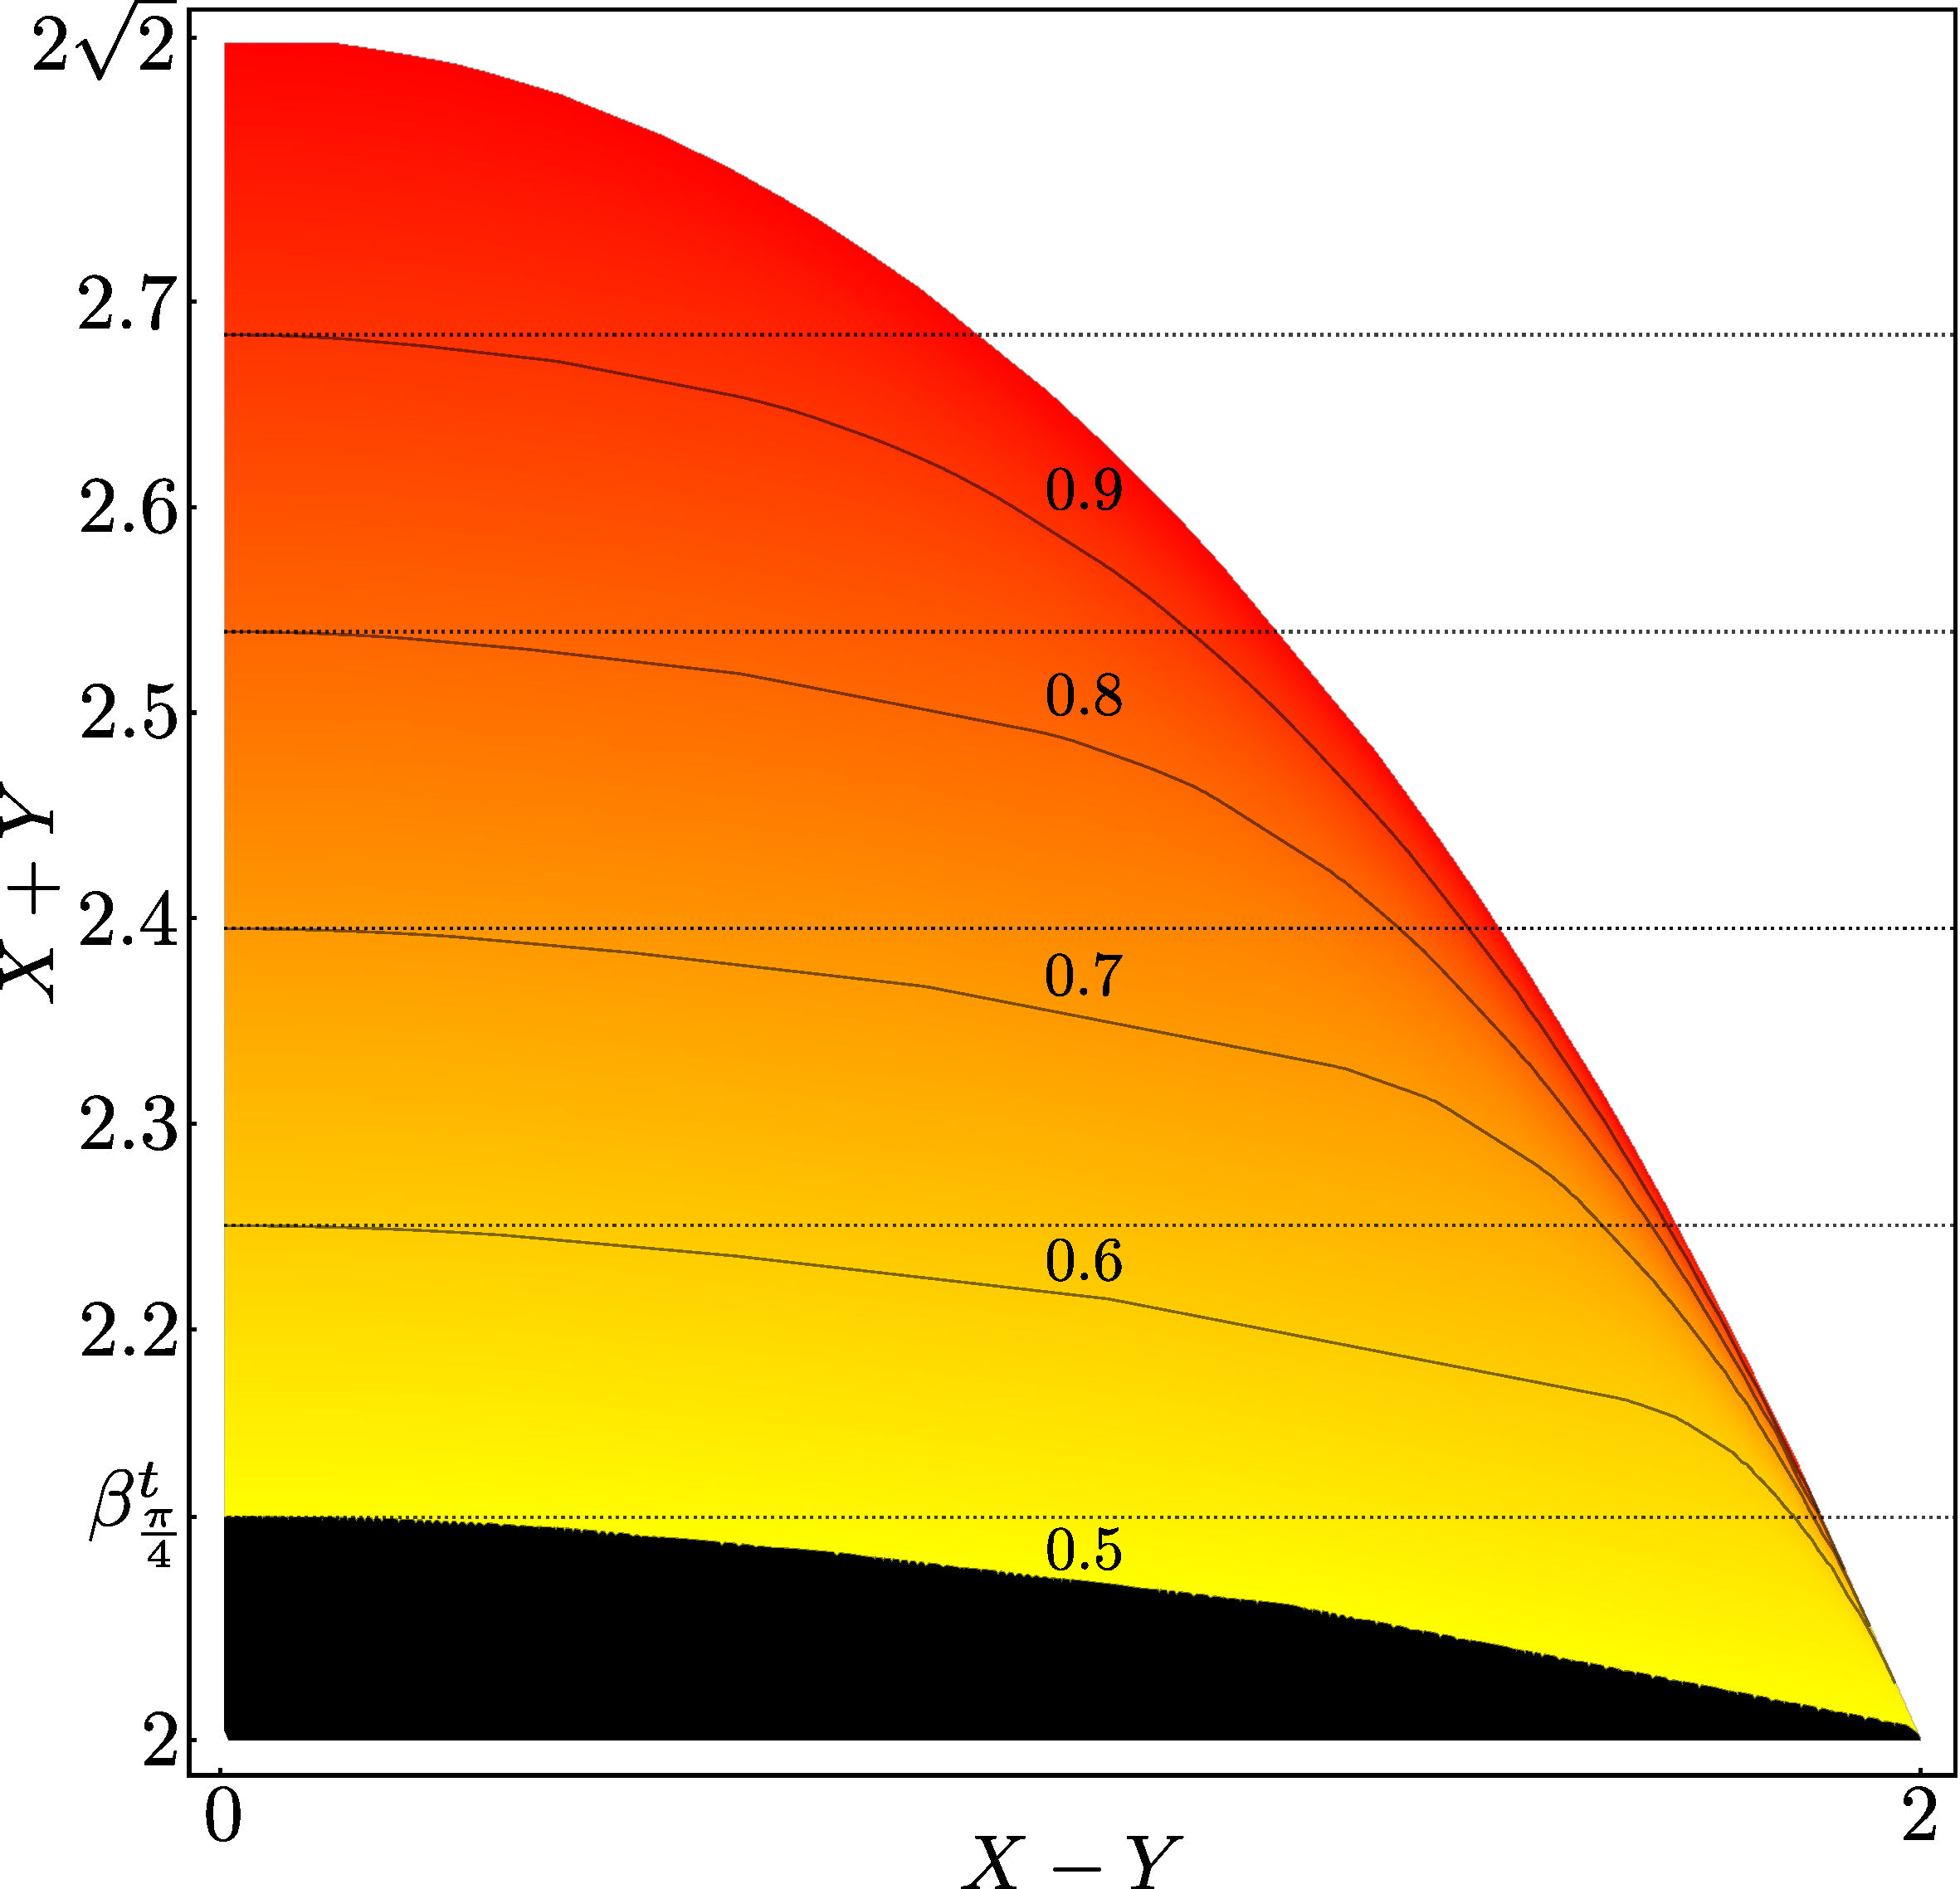
\includegraphics[width=0.95\textwidth]{chapters/selftesting/img/generalizedCHSH.pdf}
	\end{center}
	\caption{Solution to \refeq{singlet-extractability-theta} for all pair of correlator $(X,Y)$. The dashed lines represent different singlet-extractabilities using CHSH, while the solid line shows the singlet-extractability achieved using the most fitting generalized CHSH inequality. Correlators in the black zone can not be used to make self-testing statement with our method.}
	\label{fig:generalizedCHSHfid}
\end{figure}

